\documentclass[pdf]{beamer}

\usepackage[utf8]{inputenc}
\usepackage[T1]{fontenc}
\usepackage{graphicx}
\usepackage{tabto}
\usepackage{listings} % Required for insertion of code
\usepackage{tcolorbox}
\usepackage{subcaption}
\usepackage{dirtytalk}
\usepackage[main=greek, english]{babel} % For Greek language

\newcommand{\en}[1]{\foreignlanguage{english}{#1}}
\newcommand{\src}[1]{{\tt\en{#1}}}

\newcommand{\img}[1]
{
  \begin{center}
      \fcolorbox{black}{white}{\includegraphics[height=\textwidth]{#1}}
  \end{center}

}

\beamertemplatenavigationsymbolsempty

\usetheme{Madrid}

\makeatletter
\setbeamertemplate{footline}{%
\leavevmode%
\hbox{%
  \begin{beamercolorbox}[wd=.35\paperwidth,ht=2.25ex,dp=1ex,center]{author in head/foot}%
    \usebeamerfont{author in head/foot}\insertshortauthor\expandafter\ifblank\expandafter{\beamer@shortinstitute}{}{~~(\insertshortinstitute)}
  \end{beamercolorbox}%
  \begin{beamercolorbox}[wd=.60\paperwidth,ht=2.25ex,dp=1ex,center]{title in head/foot}%
    \usebeamerfont{title in head/foot}\insertshorttitle
  \end{beamercolorbox}%
}%
\begin{beamercolorbox}[wd=.2\paperwidth,ht=2.25ex,dp=1ex,right]{date in head/foot}%
  \usebeamerfont{date in head/foot}%
  \usebeamertemplate{page number in head/foot}%
  \hspace*{2ex} 
\end{beamercolorbox}
\vskip0pt%
}
\makeatother

\title{Βάσεις Δεδομένων - Εφαρμογή εθελοντικού οργανισμού}
\date{}
\author{Ευάγγελος Λάμπρου\and Ιωάννα Γέμου}

% \usebackgroundtemplate%
% {%
%     \includegraphics[height=\paperheight]{./template_beamer.png}%
% }

\begin{document}

\begin{frame}
  \maketitle
\end{frame}

\begin{frame}
  \frametitle{Θέμα της εργασίας μας}
  Δημιουργία εφαρμογής εθελοντικού οργανισμού.\\
  Βήματα που ακολουθήσαμε:
  \begin{itemize}
      \item Δημιουργία \en{ERD} και \en{Relational Schema}
      \item Κατασκευή της βάσης και εισαγωγή δεδομένων σ" αυτή
      \item Υλοποίηση του \en{Website} 
  \end{itemize}
  
\end{frame}

\begin{frame}
  \frametitle{Διάγραμμα Οντοτήτων-Συσχετίσεων}
  \begin{figure}
      \centering
      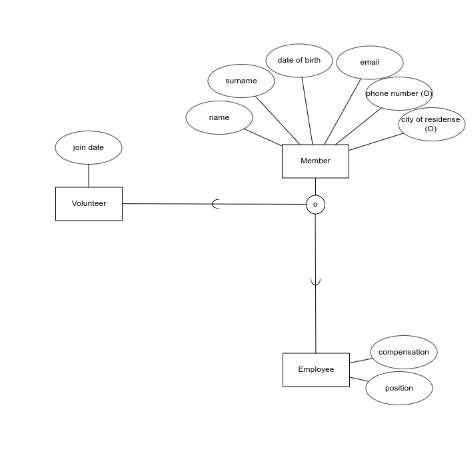
\includegraphics[width=.5\textwidth]{./images/member.png}
      \caption{\en{Superclass Member }}
  \end{figure}
  
  

\end{frame}


\begin{frame}
  \frametitle{Διάγραμμα Οντοτήτων-Συσχετίσεων}
  \begin{figure}
      \centering
      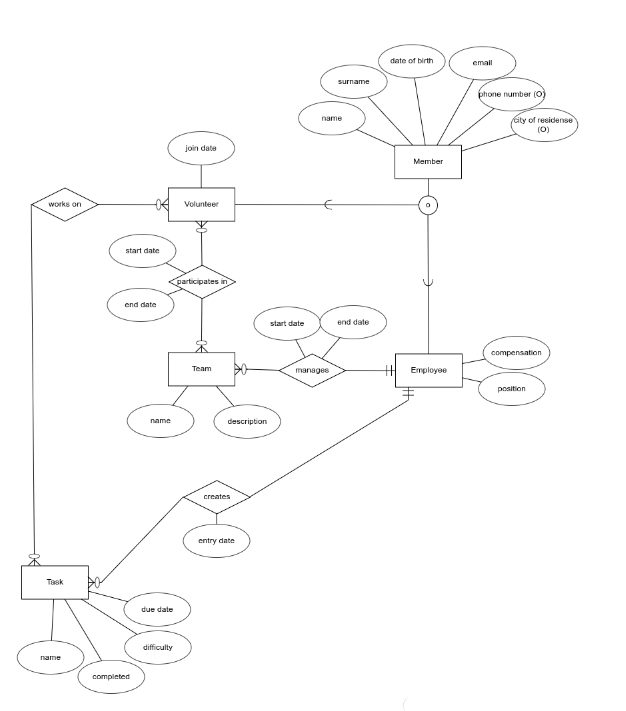
\includegraphics[width=.5\textwidth]{./images/team.png}
      \caption{\en{Team-Tasks Relationships}}
  \end{figure}

\end{frame}

\begin{frame}
  \frametitle{Διάγραμμα Οντοτήτων-Συσχετίσεων}
  \begin{figure}
      \centering
      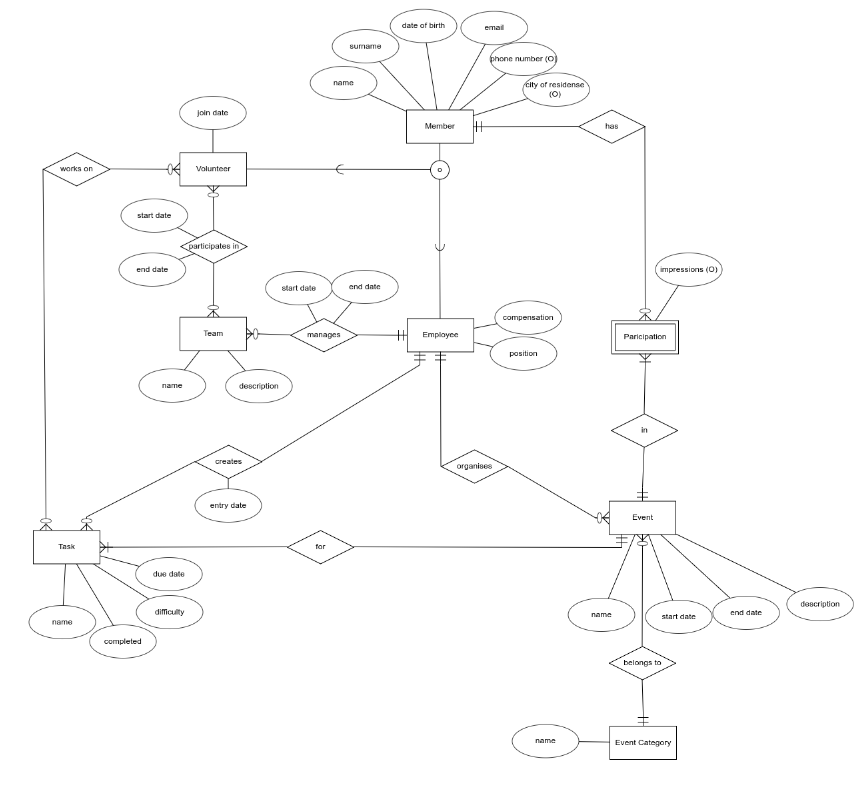
\includegraphics[width=.5\textwidth]{./images/event.png}
      \caption{\en{Event}}
  \end{figure}

\end{frame}

\begin{frame}
  \frametitle{Διάγραμμα Οντοτήτων-Συσχετίσεων}
  \begin{figure}
      \centering
      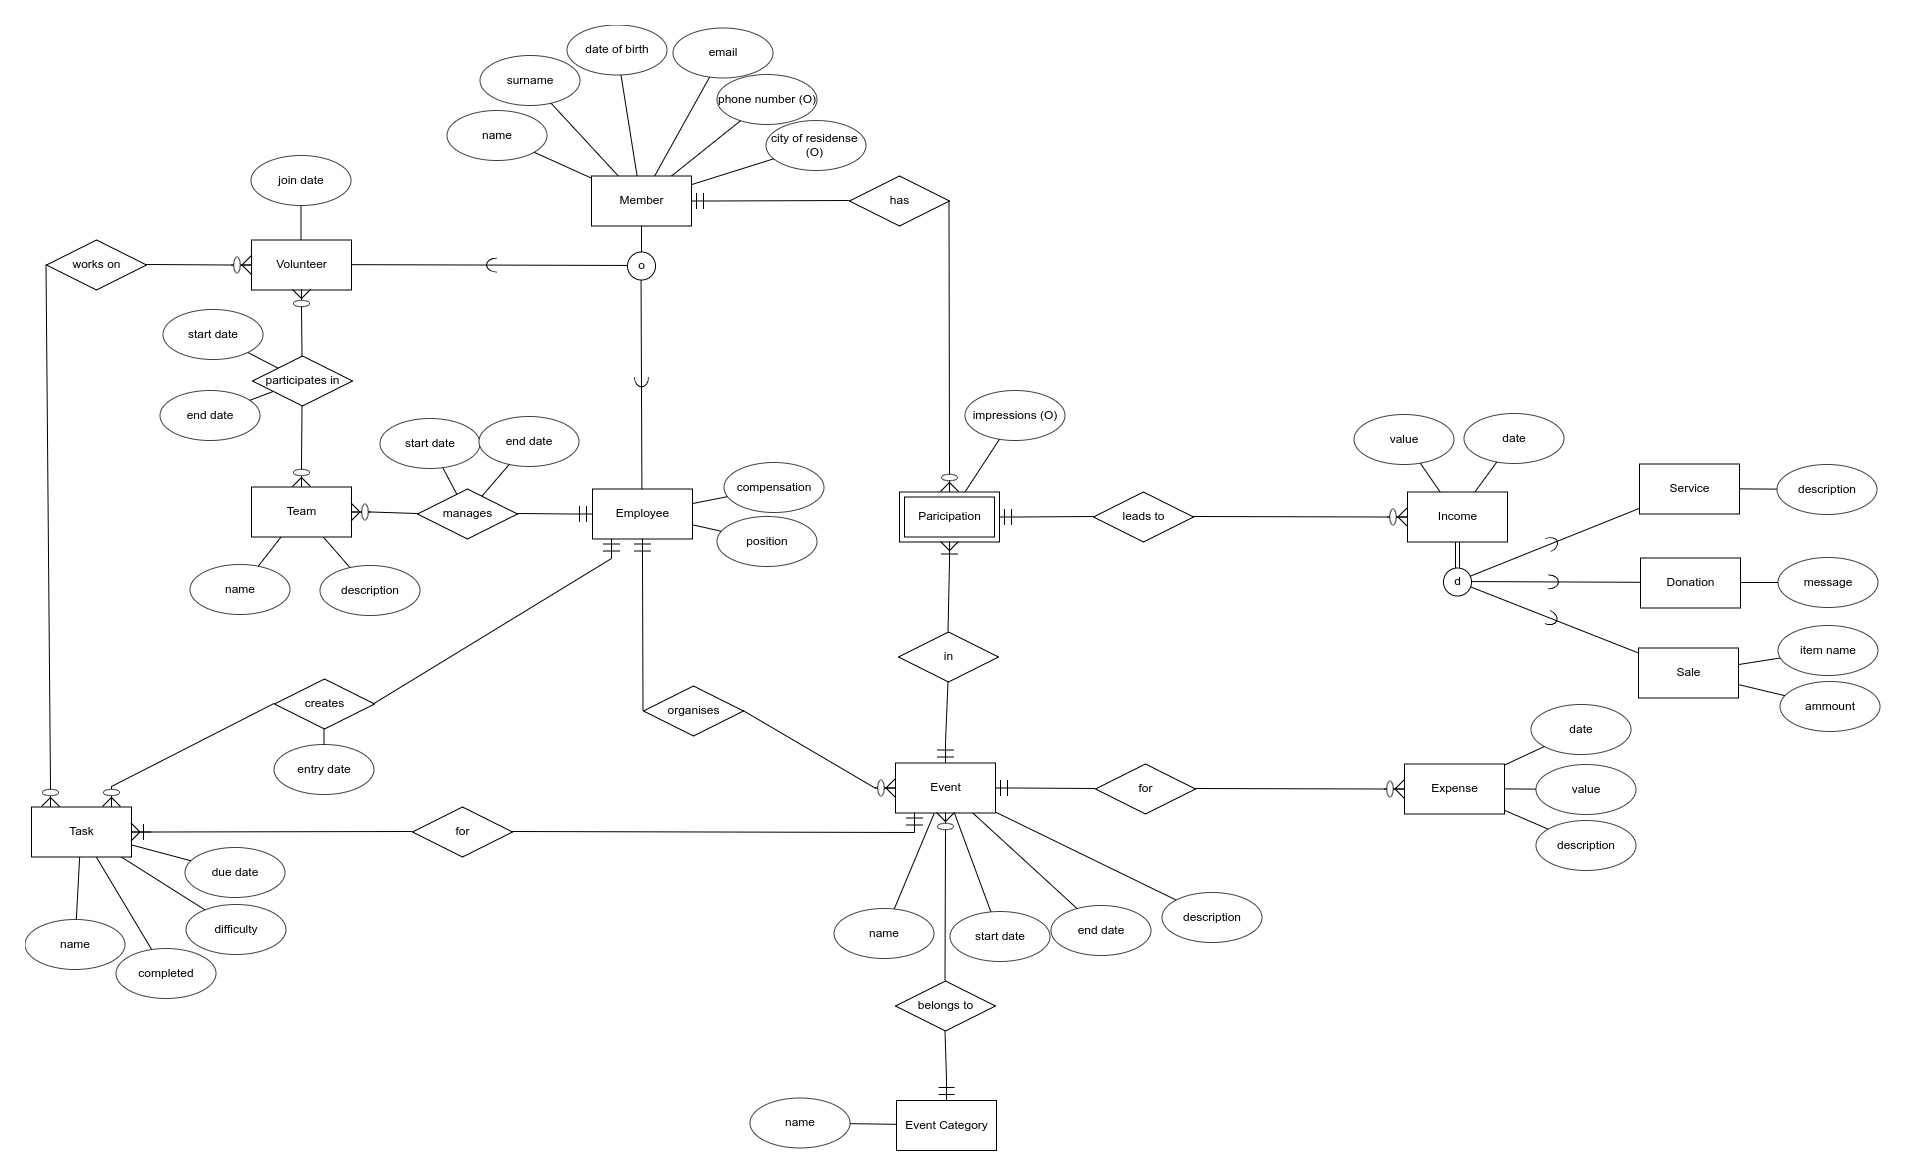
\includegraphics[width=\textwidth]{./images/erd.png}
      \caption{\en{ERD}}
  \end{figure}

\end{frame}

\begin{frame}
  \frametitle{Σχεσιακό Σχήμα}
  \begin{figure}
      \centering
      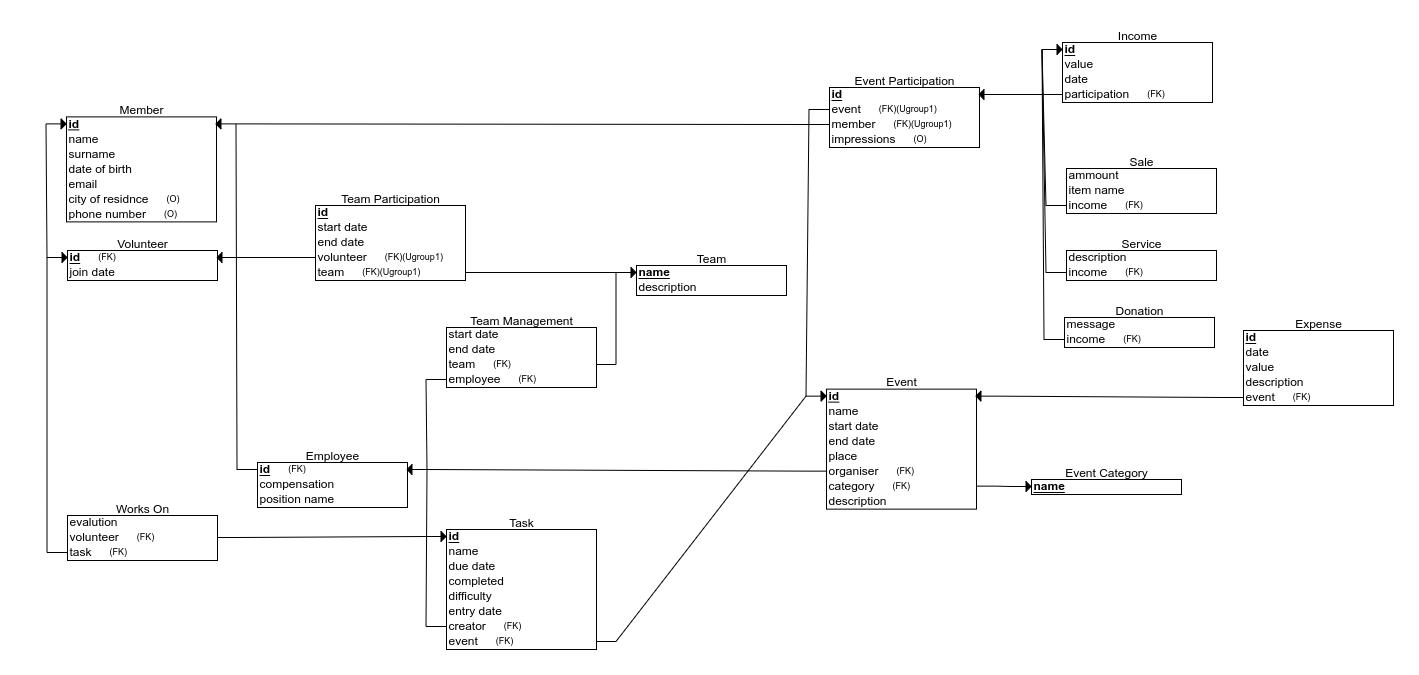
\includegraphics[width=\textwidth]{./images/schema.png}
      \caption{\en{Schema}}
   \end{figure}
  
\end{frame}




\begin{frame}
  \frametitle{}
  \centering Ευχαριστούμε για την προσοχή σας!

\end{frame}


\end{document}

